%%=============================================================================
%% Methodologie
%%=============================================================================

\chapter{\IfLanguageName{dutch}{Methodologie}{Methodology}}%
\label{ch:methodologie}

\section{Inleiding}

Voor het analyseren van het performantieverschil tussen REST en gRPC is er voor beide technologie\"en een server nodig die een API aanbiedt dat geconsumeerd kan worden en
een client die deze server aanroept. Bij dit onderzoek zal de focus niet gelegd worden op het bekomen van benchmark testen waarbij alle factoren die invloed kunnen hebben
zoveel mogelijk vermeden of uitgeschakeld worden. Er wordt getracht een realistisch scenario na te bootsen waarbij, voor de in de praktijk,
essenti\"ele stappen van zowel REST als gRPC ook effectief uitgevoerd worden.
De grootte van de verzonden dataset tegenover de tijdsduur tussen de start en einde van de request, m.a.w. tussen het aanroepen van het API door de client
tot het moment waarop alle gevraagde data bij de client toegekomen is, vormt het belangrijkste vergelijkingspunt.
Er zullen verschillende datasets verstuurd worden opdat kan worden ge\"evalueerd in hoeverre deze grootte een impact heeft op de performantie.
Aangezien er in de praktijk meestal een limiet wordt gezet op de toegelaten reponse body size wordt ook het effect van paginatie in beschouwing genomen.
Voor REST zal het veel gebruikte JSON dienen als data formaat. Hiernaast zal, met als doel de performantie te optimaliseren,
tevens naar een gecomprimeerd formaat gekeken worden. gRPC zonder gebruik te maken van het serialisatieproces lijkt in de praktijk weinig zinvol te zijn waardoor het geen onderdeel
zal uitmaken van dit vergelijkend onderzoek. Tot slot zal de performantie van gRPC middels een Stream ook vastgelegd worden.\\

\section{Opzet}
\label{sec:opzet}

Zowel de server als client applicatie worden, in aparte modules, in \'e\'en groot Gradle project geplaatst, volgens de principes van Clean Architecture. Hoewel dit
voor een kleine benchmark applicatie wat overkill lijkt, worden zoveel mogelijk best practices gevolgd. Elke applicatie start immers klein.
Gradle is een build automation tool dat ook dependency management verzorgt, waardoor het als alternatief geldt voor Maven en Ant.
Deze twee modules kunnen apart gebuild en gedeployed worden.\newline
~\autocite{Gradle}\\

\paragraph{Server applicatie}

Voor alle stadia van het onderzoek wordt er gebruikgemaakt van een Java server applicatie die zowel een REST en gRPC API aanbiedt.
In dit geval zal het gaan om API's die toelaten een lijst van fictieve personen op te vragen. Het aantal personen dat verzonden wordt, moet door de client worden aangegeven.
De eerste keer dat een lijst wordt opgevraagd, zal de data worden gegenereerd en opgeslagen in het geheugen van de applicatie volgens het aantal gevraagde objecten.
Op deze wijze is er zekerheid dat het genereren van de data slechts op de 1e maal dat het API wordt aangeroepen een vertragend effect zal hebben.
Een persoon instantie bevat 5 variabelen die tijdens het genereren van de data m.b.v.\ RandomStringUtils~\parencite{RandomStringUtils}
en RandomDataGenerator~\parencite{RandomDataGenerator} van Apache Commons opgevuld worden met willekeurige tekst of cijfers naargelang het type van variabele.
Voor elk gevraagd aantal zal de eerste request als opwarming dienen en niet gebruikt worden als vergelijking.\\

De Java applicatie wordt ontwikkeld met behulp van het Quarkus framework. Quarkus geldt als Cloud-Native Java omdat het een aantal pijnpunten van legacy
Spring en SpringBoot projecten tackelt. Bij de opkomst van Cloud Computing hadden de meeste Java applicaties problemen met resources en start-up tijden.
Spring en SpringBoot applicaties hebben voornamelijk bij de opstart heel veel geheugen nodig, waardoor dit ook moet gereserveerd blijven wanneer de applicatie aan het draaien is.
Hierdoor wordt geen effici\"ent gebruik van middelen gemaakt, met ook hogere kosten als gevolg. Quarkus (en andere Cloud-Native Java frameworks) kent ook een, in vergelijking met Spring,
zeer korte opstarttijd door bijvoorbeeld (in combinatie met GraalVM) ahead-of-time compilatie te voorzien en dode code te verwijderen.
Praktisch kunnen opstarttijden gereduceerd worden tot een paar milliseconden, alsook worden de executables (meestal docker images) kleiner.
Hierdoor kan Java in de cloud weer concurrentie aangaan met scripting-talen zoals Python en TypeScript. Deze hebben nl. niet dezelfde opstart moeilijkheden als Java.
Tot slot biedt Quarkus zowel ondersteuning voor REST als voor gRPC, een primaire vereiste voor deze applicatie.\newline
~\autocite{reasonQuarkus,whatisQuarkus,reasonQuarkus2,quarkusAbout}\\

Voor de REST API maakt Quarkus gebruik van RESTEasy, een Jakarta REST-implementatie. Jakarta REST is een REST API-standaard voor Java.
Het serialisatieproces naar JSON gebeurt d.m.v Jackson en verloopt automatisch door het Quarkus framework.
Het framework voorziet normaal ook in de mogelijkheid om de data te comprimeren alvorens ze te verzenden.
Het JSON serialisatieproces, de compressie en decompressie voor REST alsook het serialisatie- en compressieproces bij gRPC zullen telkens opnieuw moeten gebeuren.
Deze processen moeten immers ook deel uitmaken van het vergelijkend onderzoek.\newline

Het REST API wordt voorzien via de klasse People5Resource. Via de @Path annotatie voorzien van de ''/people5'' url, welke boven de klasse moet geplaatst worden,
kan aan het framework aangegeven worden welke requests tot hier geleid moeten worden.
Er worden 3 endpoints aangeboden in dit REST API die zullen aangeroepen worden tijdens de testen. Een GET endpoint ''/people5/\{amount\}'' waarmee een gespecificeerde hoeveelheid
personen kan opgevraagd worden. Dit komt overeen met de methode people5 welke ook voorzien wordt van een @Path annotatie
die het deel van de url, voor dat endpoint, meekrijgt als value nl. ''/\{amount\}''. Amount is een path variable. In de method signature moet de variabele ''amount''
ook geannoteerd worden met @PathParam met hetzelfde value als in de url om het framework deze te laten doorgeven.
Dankzij deze path variable worden bijvoorbeeld 5 personen opgevraagd via een GET request door middel van een variabele in de URI te voorzien bv.
''people/5'' of ''people/5/compressed''.
Een @GET annotatie wijst aan dat enkel requests met de GET HTTP method naar deze methode geleid mogen worden.
@Produces zegt welk media type dit endpoint zal retourneren, hier is dat application/json voor het endpoint zonder compressie, en application/octet-stream voor het endpoint voorzien van compressie.
Quarkus zal de serialisatie automatisch verzorgen. Tot slot annoteren we de method met @Uncompressed om zeker te zijn dat Quarkus hier geen compressie zal toepassen.
Een tweede GET endpoint ''/people5/\{amount\}/compressed'' heeft grotendeels dezelfde werking, maar de data wordt gecomprimeerd alvorens ze wordt verzonden.
Deze wordt met de people5compressed methode gedefinie\"rd. \newline
Tijdens het implementeren van beide applicaties bleek Quarkus, ondanks het volgen van de tutorial van Quarkus~\parencite{quarkusgzipcompressie}
en een oplossing van een GitHub discussie~\parencite{quarkusgzipcompressiegithub} uit te proberen, de compressie niet uit te voeren.
Hierdoor is er gekozen de gzip compressie simpelweg zelf te implementeren middels een gzip methode welke grotendeels gebaseerd is op een gevonden voorbeeld van Java2s~\parencite{gzipCompressie}.
Deze methode aanvaard een Lijst van generieke objecten en geeft een byte array terug welke de gecomprimeerde data bevat.\newline
Via het derde endpoint kan de opgeslagen data, ook cache genaamd, worden leeggemaakt. Dit endpoint kan aangeroepen worden via een POST request naar
de URI van de applicatie aangevuld met ''/people5/cleardata''. Hier worden ook weer een @Path annotatie voorzien met ''/cleardata'', een @POST annotatie om de HTTP method te
specifi\"eren en nog een @Produces met ''application/json'' voor het data formaat aan te geven. Indien de cache wordt leeggemaakt is dit voor beide beschikbare formaten van toepassing.
Dit endpoint geeft een lijst terug met de eerder gevraagde hoeveelheden die nu in de cache zitten.
Na het leegmaken van de cache zou dit dus steeds een lege lijst moeten zijn.\newline
~\autocite{quarkusREST,Jakarta}\\

Voor het gRPC API wordt gestart vanaf de Quarkus ''tutorial Getting Started With gRPC''~\parencite{quarkusgRPC}.
Bij gRPC moet er een bestand gemaakt worden, met .proto als extensie, waarin alle procedures, welke ter beschikking zijn, worden vastgelegd.
Op basis van dit bestand zal de protocol buffer compiler code genereren.

Het bestand, waarvan een voorbeeld weergegeven wordt in figuur~\ref{fig:protobestand}, start met aan te geven welke syntax van de protocol buffers gebruikt wordt, in dit geval, de meest recente versie nl. versie 3.
Daarna volgen drie opties die specifiek voor Java applicaties dienen: ''java\_multiple\_files'', ''java\_package'' en ''java\_outer\_classname''.
java\_multiple\_files staat op true zodat er een apart .java bestand gemaakt wordt voor elke gegenereerde klasse in plaats
van één wrapper klasse en daarbij, in geneste klassen, alle andere klassen. Bij ''java\_package'' staat niet dezelfde package die in de rest van de applicatie gebruikt is,
maar wordt een proto subpackage opgegeven, waarmee de best practices gevolgd worden.
Tot slot geeft de ''java\_outer\_classname'' optie aan dat People5GrpcProto moet gebruikt worden als naam voor de wrapper klasse van de service gedefinieerd in dit .proto bestand.
Daaronder wordt aangegeven welk package wordt gebruikt voor de gegenereerde code. Dit wordt overschreven door de ''java\_package'' optie die eerder gedefinieerd werd maar
in de protobuf Java tutorial~\parencite{protobufJava} wordt vermeld dat er steeds een package moet gedefinieerd worden, zelfs bij het gebruik van de optie jav\_package, om naam collisie
te vermijden in de protocol buffer name space.\newline
Nu volgt de effectieve beschrijving van het gRPC API startend met een service interface genaamd People5Grpc waarin
alle beschikbare functies worden gedefinieerd. De functie ClearData werkt zoals het eerder beschreven gelijknamige REST endpoint en zorgt dat de cache wordt leeggemaakt.
Met de functie GetPeople kan een lijst van persoon-objecten opgevraagd worde, de grootte van de lijst komt overeen met de opgegeven hoeveelheid.
Tot slot is er een GetPeopleStream functie die een stream van persoon-objecten teruggeeft van het gevraagde aantal.\newline
Na deze functies gedefinieerd te hebben moeten de messages die ze ontvangen en verzenden omschreven worden.
ClearDataInput en SupportedAmountsInput zijn lege messages. Er moet steeds een message opgegeven worden voor het return value van een functie.
In plaats van een lege message te defini\"eren kan ook google.protobuf.Empty gebruikt worden, maar dan is het achteraf niet mogelijk om de bestaande functie
te wijzigen in die zin dat ze toch een niet lege message meegeeft. Door een message te beschrijven kunnen hier later nog variabelen aan toegevoegd worden.
Voor dit onderzoek zal dit waarschijnlijk niet nodig zijn maar er wordt toch geopteerd de best practices te respecteren.
SupportedAmounts bevat een lijst van integers, dit wordt aangegeven door het keyword repeated.
Net zoals bij het REST endpoint cleardata zou deze lijst steeds leeg moeten zijn gezien de cache juist werd leeggemaakt.
De message GrpcPeople5 bevat een lijst van GrpcPerson5 messages. GrpcPerson5 geeft het persoon object weer en definieert de 5 variabelen. Als laatste message is er nog
Amount dat als te ontvangen message dient voor de GetPeople en GetPeopleStream functies. Deze message omvat simpelweg een integer die aangeeft hoeveel persoon objecten moeten
verzonden worden.\newline
Op basis van dit .proto bestand zullen de nodige klassen gegenereerd worden, in figuur~\ref{fig:gegenereerdeklassengrpc} wordt een afbeelding weergegeven.
Dit gebeurd tijdens het build proces van Gradle door het commando ''graldew build -x test''.
Deze klassen zijn terug te vinden in de folder ''\textbackslash{}build\textbackslash{}classes\textbackslash{}java\textbackslash{}main'' van de entrypoints-grpc module onder application-server,
in het Java package be.hogent.nthiers zoals opgegeven met de java\_package optie. De gegenereerde interface People5Grpc moet nu in de applicatie zelf ge\"{\i}mplementeerd worden.
Hier zal de gRPC API functionaliteit gekoppeld worden aan de achterliggende logica met name de GrpcPeopleCache. De 3 methodes die People5Grpc defineert komen overeen met de 3 functies die
in het .proto bestand zijn opgegeven. Hun return value en method variables zijn ook gegenereerde klassen die de messages van het .proto bestand weerspiegelen.
Deze zijn voorzien van een builder waarmee we ze kunnen construeren.\newline
Het gRPC API maakt gebruik van de gegenereerde GrpcPerson5 klasse en dus niet dezelfde klasse als REST. Hierdoor wordt er voor het gRPC API een andere cache gebruikt dan
die van het REST API. Indien dezelfde zou gebruikt worden zouden de Person5 objecten gebruikt voor REST voor de gRPC calls steeds naar GrpcPerson5 objecten gemapt moeten worden
wat de performantie mogelijks negatief zou impacteren. Er zou kunnen geopperd worden dat het omzetten van het domein object naar de gegenereerde klasse bij een gRPC API steeds nodig
zal zijn en er dus ook rekening mee gehouden dient te worden bij het evalueren van de performantie, het is echter ook bij REST best practice om het domein niet rechtstreeks
via een API bloot te stellen, maar daarentegen om te zetten naar zogenaamde data transfer objects.\newline
~\autocite{quarkusgRPC,DTO,gRPCBestPractices,builderPattern}\\

\begin{figure}[ht]
    \centering
    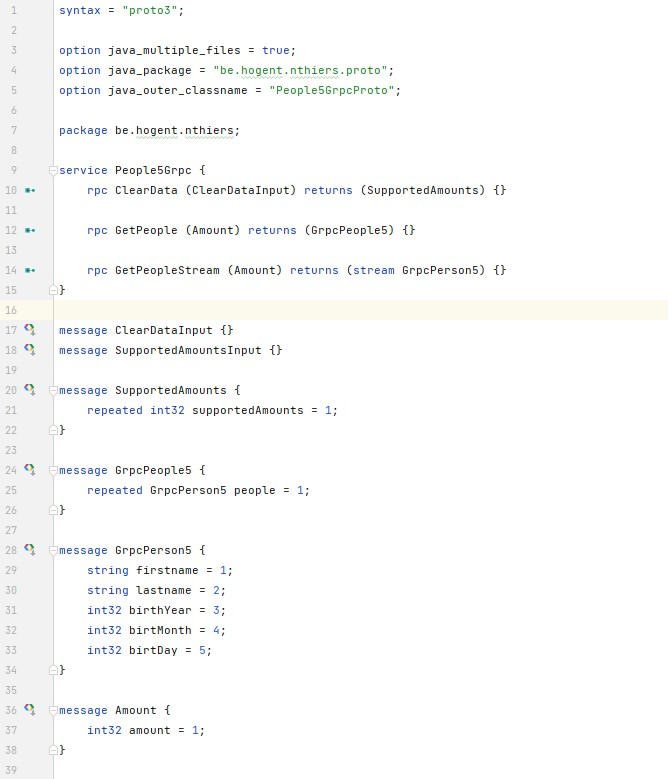
\includegraphics[width=1.0\linewidth]{protobestand}
    \caption{.proto bestand}
    \label{fig:protobestand}
\end{figure}

\begin{figure}[ht]
    \centering
    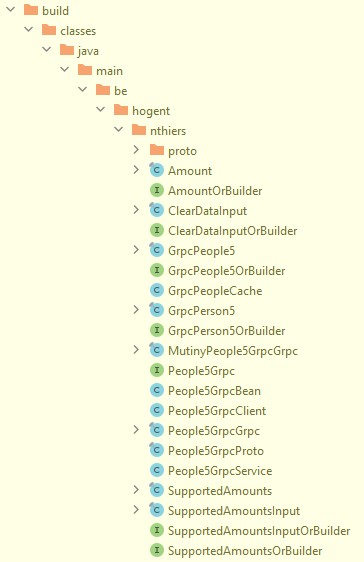
\includegraphics[width=1.0\linewidth]{gegenereerdeklassengrpc}
    \caption{Door protocol buffer compiler gegenereerde klassen}
    \label{fig:gegenereerdeklassengrpc}
\end{figure}

Als deployment platform, is er geopteerd om OpenShift te gebruiken. OpenShift geldt als een enterprise ready Kubernetes cluster.
Een Kubernetes cluster is een orchestration tool voor container platforms met onderliggend een set van gelinkte servers (nodes)
waarop containerized applicaties gedeployed kunnen worden.
Entreprise ready duidt op het feit dat OpenShift reeds in een aantal functionaliteiten (security, stabiele upgrades, stabiliteit, \ldots)
voorziet, zodat de configuratie opzet en het deployment proces makkelijker verlopen.
Hierdoor zou er sneller moeten gestart kunnen worden met het echte doel nl. het hosten en deployen van de applicatie.
OpenShift heeft ook een administrator en developer view, waarbij vooral de developer view het gemakkelijk maakt om applicaties te gaan deployen
zonder de interne werken van Kubernetes door en door te moeten kennen.
Tot slot biedt Red Hat een gratis sandbox aan om een maand lang mee te werken. Verder in de tekst wordt met OpenShift of Kubernetes beiden gerefereerd naar de deploy omgeving
omdat OpenShift uiteindelijk ook gewoon Kubernetes is.\newline
~\autocite{redhatwhatiskubernetes,redhatopenshiftkubernetes,redhatopenshift}\\

Om een microservice met een REST API in Kubernetes opgezet te krijgen, zijn er drie configuratie bestanden nodig: een deployment config,
een service config en een route config.~\parencite{openshiftDeployment}
\begin{itemize}
    \item Deployment config: bevat onder andere de docker image die gebruikt moet worden, de namespace en de resource reservations zoals geheugen en CPU.
    \item Service config: is de interne DNS binnen Kubernetes en laat applicaties toe om andere applicaties via service naam aan te spreken.
    \item Route config: is een config om services extern beschikbaar te stellen. Dit houdt in dat er van buiten de Kubernetes cluster connectie met de deployment kan gemaakt worden.
\end{itemize}

Kubernetes deployments zijn eenvoudig in een REST context. Voor gRPC blijkt het toch uitdagender te zijn door de harde dependency van gRPC op TLS/SSL.
De Kubernetes/OpenShift routes moeten ook geconfigureerd worden om, in plaat van op de Ingress controllers, TLS
verificatie over te laten aan de deployments (i.e., containers/PODs), dus de applicatie zelf. Dit vereiste in een eerste stap dat TLS terminatie van de route
geconfigureerd werd als ''passthrough'' in plaats van ''edge''.

Daarenboven zijn er ook gevalideerde certificaten noodzakelijk doordat gRPC geen manueel getekende certificaten toelaat.
Hiervoor wordt er gebruikgemaakt van Let's Encrypt om certificaten te genereren.
OpenShift/Kubernetes kent het concept van operators: dit zijn componenten binnen de cluster die heel wat infrastructuur werk overnemen.
Bepaalde installaties (bv. Kafka, cert manager, \ldots) worden hierdoor beschikbaar op verzoek.
Zo kan een cert-manager operator ge\"{\i}nstalleerd, een issuer geconfigureerd en een certificate request gegenereerd worden.
Deze request wordt dan opgeslagen in een Kubernetes secret en ge\"{\i}njecteerd in een Kubernetes/OpenShift deployment.
Op deze manier krijgt de applicatie direct de nieuwe certificaten toegewezen.
De verschillende resource files zullen kunnen worden teruggevonden in de folder ''application\_server\textbackslash{}configuration\textbackslash{}metadata''.

De server applicatie werd gedeployed naar OpenShift van Red Hat. Op OpenShift is HTTP 2 en dus ook gRPC connectiviteit steeds met gebruik van het TLS protocol.
Gezien het gebruik van TLS bij gRPC ook als best practice gezien wordt, zoals eerder gemeld in de stand van zaken, zal het hier mee onderdeel uitmaken van performantie testen.\newline
~\autocite{openshifttls}

\paragraph{Client applicatie}

De client applicatie zal klassen voorzien die zowel het REST als gRPC API kunnen aanspreken.
Net zoals bij de server applicatie maakt de client applicatie gebruik van Quarkus.\\

Voor de REST client wordt een interface bij Quarkus kenbaar gemaakt als REST client door middel van de @RegisterRestClient annotatie. Deze annotatie wordt ook een configKey meegeven
zodat Quarkus weet welke configuratie moet gebruikt worden voor deze client.  Enkel de url en scope properties zijn hierbij nodig waarbij de url slaat op de url van de
REST API die wordt aangesproken en de scope aangeeft welke CDI scope deze client dient te krijgen, in dit geval Singleton.
Verder wordt de interface zelf voorzien van de @Path annotatie met als String value een deel van de url welke
aan alle endpoints gemeen is, meer specifiek ''/people5''. Elke methode die voorzien wordt in de interface staat voor een endpoint dat kan aangesproken worden.
Boven de clearData methode staat een @POST annotatie waarmee wordt aangegeven dat bij deze methode de POST HTTP-method moet gebruikt worden alsook
nog een @Path annotatie met ''/cleardata'' als value die de url verder specificeert. De people5 methode krijgt een @GET en een @Path annotatie, waarbij die laatste ''/\{amount\}''
als value heeft. Deze methode heeft een parameter amount welke ook voorzien wordt van een @PathParam annotatie met ''amount'' als value zodat Quarkus
deze parameter als path parameter zal gebruiken. De derde methode people5Compressed is buiten de naam identiek als de people5 methode maar hier gaat het endpoint een
byte array ontvangen wat aangegeven wordt door de @Consumes annotatie voorzien van ''application/octet-stream''. Het omzetten van de byte array naar de Java objecten gebeurt
in de test klasse, door middel van de methode gzipDecompressBytes, die gebaseerd is op een simpel voorbeeld van java2s~\parencite{gzipDecompressie},
De methode ontvangt een byte array en geeft lijst van generieke objecten terug en zal nog mee onderdeel zijn van performantiemetingen,
ze wordt dus uitgevoerd alvorens het ontvangen van de data geregistreerd wordt in de TestHelper klasse.
~\autocite{quarkusRESTclient}\\

Voor de gRPC client moet weer een .proto bestand voorzien worden op basis waarvan de protocol buffer compiler de nodige code kan genereren. Gemakkelijkheidshalve wordt het
.proto bestand van de server applicatie hier gewoon gekopieerd. In tegenstelling tot in de server applicatie moet er hier geen interface ge\"{\i}mplementeerd worden maar
is er door de code generatie een People5Grpc klasse beschikbaar waarmee het gRPC API van de server kan worden aangesproken. Deze klasse kan door gebruik van de
@GrpcClient annotatie ge\"{\i}njecteerd worden in de service klasse welke de functionaliteit verder zal implementeren voor gebruik door de testen. Deze annotatie
kan voorzien worden van een String value element name die door Quarkus zal gebruikt worden om de gRPC client te configureren. In de properties worden enkele properties voorzien
die Quarkus nodig heeft. Quarkus weet dankzij de opgegeven element name welke properties hij voor deze specifieke client moet gebruiken.
\begin{itemize}
    \item ''use-quarkus-grpc-client'' wordt op false gezet zodat de gRPC implementatie gebaseerd op Netty gebruikt wordt. Deze werkt op OpenShift.
    \item ''port'' dient om de poort aan te geven via welke de communicatie met het gRPC API zal gebeuren
    \item ''host'' laat toe de url te defini\"eneren van de gRPC server
    \item ''ssl.certificate'' geeft de naam van het SSL certificaat welke zich in de recources folder van de client applicatie bevindt
    \item ''max-inbound-message-size'' wordt gebruikt om de standaard maximum message grootte van 4MB te wijzigen
\end{itemize}

Om de gRPC client People5Grpc aan te spreken moeten dezelfde gegenereerde message klassen gebruikt worden als in de server applicatie.
De clearData en de getPeople methode hebben beiden de wrapper klasse ''io.smallrye.mutiny.Uni'' als return type respectievelijk met de gegenereerde klassen
SupportedAmount en GrpcPeople5, deze laatste bevat een lijst met GrpcPerson5 objecten. De getPeopleStream methode daarentegen geeft een ''io.smallrye.mutiny.Multi'' terug.
Zowel Uni als Multi representeren een stream en zijn asynchrone types. Uni omvat slechts één item of een fout. Multi omvat 0 tot potentieel oneindig veel items.
Voor Uni zal er gewoon op het item gewacht worden tot dit ontvangen is. Voor een Multi zal er gesubscribed worden en zullen er drie functies nodig zijn om
de items te verwerken. De eerste functie, van het type Consumer~\parencite{Consumer}, gaat elk item verwerken, de tweede functie, weer het type Consumer~\parencite{Consumer},
gaat eventuele failures verwerken en de derde functie, van het type Runnable~\parencite{Runnable} wordt aangeroepen wanneer de call voltooid is.\newline
~\autocite{quarkusgRPCclient,SmallRyeMutiny,MultiSubscribing}\\

De performantie testen worden in dit deel van het project voorzien. De testklasse People5RestServiceTest omvat de performantietesten voor het REST API
en de People5GrpcServiceTest omvat de testen voor het gRPC API. Beiden maken gebruik van een hulp klasse TestHelper de oproepen naar de API's gaat doen,
logs gaat bijhouden en ook het tijdsverloop registreren. Voor de constructie van deze hulp klasse moeten drie parameters meegegeven worden nl. een functie
die kan aangeroepen worden om de cache leeg te maken, een object mapper die de objecten naar JSON formaat kan serialiseren en deserialiseren en tot slot de
functie die moet aangeroepen worden om de API calls te doen. Er zijn dan 2 publieke methodes, testPerformance\_singularRequests en testPerformance\_multipleRequests,
die door de testklassen worden aangeroepen. Bij testPerformance\_singularRequests moet de naam van de test meegegeven worden, deze zal bij het wegschrijven
van het logbestand en ook in de logs zelf gebruikt worden, en de lijst van aantallen, in de vorm van een lijst van integers, welke moeten opgevraagd worden
d.m.v. de API call. Eerst wordt de cache eerst leeggemaakt dan wordt de API call tweemaal uitgevoerd zodat de cache voor de specifieke call die getest moet worden
zeker opgevuld is en zodat de server opgewarmd is. Daarna wordt de performantie gemeten door de tijd te registreren en de call nogmaals uit te voeren.
Wanneer het antwoord ontvangen is, wordt de tijdsduur vastgelegd. Bij de REST calls wordt de ontvangen lijst van personen nogmaals geserialiseerd naar JSON
en naar een file weggeschreven om zo de grootte van de dataset in JSON formaat te kunnen registreren.
Tot slot gaat de TestHelper ook de logs, met daarin het resultaat van de performantietest, wegschrijven naar een file.
De tweede methode testPerformance\_multipleRequests verwacht ook de testnaam, een lijst van amounts en daarnaast nog een integer genaamd batchSize.
Tijdens het uitvoeren van deze methode zullen de opgegeven aantallen opgehaald worden door middel van de API call meermaals uit te voeren met de batchSize als aantal
tot het totale gevraagd aantal is ontvangen. Ook hier wordt de tijd geregistreerd, maar dan van het ophalen van het volledige aantal d.m.v.
verschillende calls van de opgegeven batch grootte.\\

De hele opzet in deze methodiek kan een effect hebben op de resultaten die zullen bekomen worden. Het wijzigen ervan zal dus kunnen maken dat de resultaten afwijken.
Bij het beschouwen van de hierbij geregistreerde performantie verschillen moet daar rekening mee gehouden worden. Grote verschillen en verhoudingen tussen resultaten zullen echter
ook na aanpassing van de test modaliteiten gelijkaardig blijven, waardoor het mogelijk zal zijn een conclusie te maken en voordeel te halen uit dit onderzoek.\\

De broncode van dit project, dat zowel de server als client applicatie omvat, is publiek beschikbaar op Github via https://github.com/thiersnicolas/gRPC\_vs\_REST.git

\section{Enkelvoudige requests}
\label{enkelvoudigerequestsmethodologie}

Uit de eerdere uitleg over de implementatie van de TestHelper klasse zal al enigszins duidelijk geworden zijn hoe de performantie testen gaan verlopen.
Er wordt gestart met de performantie te evalueren van enkelvoudige requests voor welbepaalde sets van data voor alle geïmplementeerde API calls.
Het doel is vast te leggen hoe de verhouding van het tijdsverloop tussen de verschillende API calls is en hoe deze evolueert naargelang de
datasets groter of kleiner zijn.\\

De API calls die zullen worden uitgevoerd:
\begin{itemize}
    \item REST API: GET people5
    \item REST API
    \item gRPC getPeople
    \item gRPC getPeopleStream
\end{itemize}

Tabel~\ref{tab:Gevraagdedatasets} geeft de datasets weer die zullen opgevraagd worden, hiervoor werd reeds gekeken wat hun grootte is
wanneer ze in JSON formaat naar een bestand worden weggeschreven (deze grootte kan zeer kleine verschillen vertonen welke nagenoeg geen impact zullen hebben op de performantie).
Alle datasets zullen vier maal opgevraagd worden waarna het gemiddelde ervan genomen wordt om de verschillende soorten API calls te gaan vergelijken.\\

\begin{table}
    \centering
    \begin{tabular}{rrll}
        \toprule
        \textbf{Aantal personen} & \textbf{Grootte (bytes)} & \textbf{Grootte (KB)} & \textbf{Grootte (MB)} \\
        \midrule
        1024 & 89028 & 86,94 & 0,08 \\
        2048 & 178062 & 173,89 & 0,17 \\
        4096 & 356103 & 347,76 & 0,34 \\
        8192 & 712225 & 695,53 & 0,68 \\
        9216 & 801209 & 782,43 & 0,76 \\
        10240 & 890124 & 869,26 & 0,85 \\
        11264 & 979136 & 956,19 & 0,93 \\
        12288 & 1068188 & 1043,15 & 1,02 \\
        13312 & 1157125 & 1130 & 1,1 \\
        14336 & 1246294 & 1217,08 & 1,19 \\
        15360 & 1335174 & 1303,88 & 1,27 \\
        16384 & 1424160 & 1390,78 & 1,36 \\
        20480 & 1780317 & 1738,59 & 1,7 \\
        24576 & 2136595 & 2086,52 & 2,04 \\
        28672 & 2492585 & 2434,17 & 2,38 \\
        32768 & 2848302 & 2781,54 & 2,72 \\
        36864 & 3204548 & 3129,44 & 3,06 \\
        40960 & 3560626 & 3477,17 & 3,4 \\
        45056 & 3916542 & 3824,75 & 3,74 \\
        49152 & 4272567 & 4172,43 & 4,07 \\
        53248 & 4628732 & 4520,25 & 4,41 \\
        57344 & 4984625 & 4867,8 & 4,75 \\
        61440 & 5341250 & 5216,06 & 5,09 \\
        65536 & 5697065 & 5563,54 & 5,43 \\
        131072 & 11394036 & 11126,99 & 10,87 \\
        262144 & 22788054 & 22253,96 & 21,73 \\
        524288 & 45575493 & 44507,32 & 43,46 \\
        \bottomrule
    \end{tabular}
    \caption{Gevraagde Datasets}
    \label{tab:Gevraagdedatasets}
\end{table}

Voor de 2 REST calls en de getPeople functie van het gRPC API is het simpelweg de lijst in tabel \ref{tab:Gevraagdedatasets} doorgeven aan de testPerformance\_singularRequests methode
van de TestHelper. De getPeopleStream methode van het gRPC API geeft een object van het type Multi terug, waarover eerder reeds meer informatie werd gegeven.
Om deze methode te testen is er een nieuwe functie gemaakt welke door middel van een AtomicInteger de tel bijhoudt van alle ontvangen items en bij het voltooien van
de gRPC functie een AtomicBoolean op true zet. Wanneer die AtomicBoolean op true staat wordt de controle teruggegeven aan de TestHelper. Tijdens het uitvoeren van
de testen bleek dat effectief alle gevraagde items ontvangen werden maar tevens dat er een significate impact was op de performantie.
Om een correcte performantiemeting te kunnen doen dient de AtomicInteger terug verwijderd te worden.
De AtomicBoolean wordt enkel en alleen gewijzigd wanneer de oproep voltooid is waardoor dit nagenoeg geen impact zal hebben.

\section{Meervoudige requests}

In deze volgende onderzoeksfase wordt er meer rekening gehouden met eventuele praktische beperkingen waarmee applicaties kunnen en zullen geconfronteerd worden.
Zo zal het beschikbare geheugen van een applicatie alsook het aantal simultane requests die mogelijks zullen ontvangen worden het noodzakelijk maken om
de toegelaten response grootte te beperken. Voor REST wordt er in dergelijke gevallen vaak voor het pagineren van datasets geopteerd.
Hierbij is de verstuurde dataset slechts een deel van het geheel. De client geeft bij een gepagineerde request aan hoe groot de subset moet zijn
en het hoeveelste deel deze subset is van de gehele dataset. De server geeft de gevraagde subset aangevuld door de subset grootte, de positie t.o.v. de gehele set
en tot slot ook de grootte van de gehele lijst.\\

Praktisch wordt hier de testPerformance\_multipleRequests van de TestHelper klasse aangeroepen voor alle REST API calls en de getPeople functie van het gRPC API.
Het tijdsverloop van alle calls, met de opgegeven batch grootte, tot de gehele dataset ontvangen is, zal worden geregistreerd. Eerst zullen verschillende batchgroottes
uitgetest worden om te evalueren wat de impact van deze grootte is op de performantie. Een grote batch heeft immers tot gevolg dat er minder calls zullen moeten uitgevoerd worden.\newline
Tabel ~\ref{tab:Batches} geeft aan welke batches zullen worden gebruikt. Het totale aantal items die worden opgevraagd bedraagt 4.194.304, met samen een grootte
van 347,68 MB wanneer ze worden weggeschreven in JSON formaat naar een bestand. De hoogste snelheid waarmee deze grote dataset, door middel van batched calls, kon worden
opgehaald zal dan vergeleken worden tussen de verschillende API's en verschillende formaten of methodes\\

getPeopleStream van het gRPC API is hier weer het vreemde eendje waarbij het pagineren van de calls zinloos is. De server zal immers de beschikbare capaciteit gebruiken
om item per item door te sturen, gebruik makend van de HTTP 2 functionaliteit, zolang de client niet blokkeert. Voor getPeopleStream zal de testPerformance\_singularRequests methode van
de TestHelper klasse gebruikt worden voor de totale grootte die ook bij de andere API calls wordt opgevraagd.
De performantie hiervan kan dan correct vergeleken worden met de andere resultaten.\\

\begin{table}
    \centering
    \begin{tabular}{rrrll}
        \toprule
        \textbf{Aantal calls} & \textbf{Items / call} & \textbf{Grootte batch (bytes)} & \textbf{Grootte batch (KB)} & \textbf{Grootte batch (MB)} \\
        \midrule
        4096 & 1024 & 89028 & 86,94 & 0,08 \\
        2048 & 2048 & 178062 & 173,89 & 0,17 \\
        1024 & 4096 & 356103 & 347,76 & 0,34 \\
        512 & 8192 & 712225 & 695,53 & 0,68 \\
        456 & 9216 & 801209 & 782,43 & 0,76 \\
        410 & 10240 & 890124 & 869,26 & 0,85 \\
        373 & 11264 & 979136 & 956,19 & 0,93 \\
        342 & 12288 & 1068188 & 1043,15 & 1,02 \\
        316 & 13312 & 1157125 & 1130 & 1,1 \\
        293 & 14336 & 1246294 & 1217,08 & 1,19 \\
        274 & 15360 & 1335174 & 1303,88 & 1,27 \\
        256 & 16384 & 1424160 & 1390,78 & 1,36 \\
        205 & 20480 & 1780317 & 1738,59 & 1,7 \\
        171 & 24576 & 2136595 & 2086,52 & 2,04 \\
        147 & 28672 & 2492585 & 2434,17 & 2,38 \\
        128 & 32768 & 2848302 & 2781,54 & 2,72 \\
        114 & 36864 & 3204548 & 3129,44 & 3,06 \\
        103 & 40960 & 3560626 & 3477,17 & 3,4 \\
        94 & 45056 & 3916542 & 3824,75 & 3,74 \\
        86 & 49152 & 4272567 & 4172,43 & 4,07 \\
        79 & 53248 & 4628732 & 4520,25 & 4,41 \\
        74 & 57344 & 4984625 & 4867,8 & 4,75 \\
        69 & 61440 & 5341250 & 5216,06 & 5,09 \\
        64 & 65536 & 5697065 & 5563,54 & 5,43 \\
        32 & 131072 & 11394036 & 11126,99 & 10,87 \\
        16 & 262144 & 22788054 & 22253,96 & 21,73 \\
        8 & 524288 & 45575493 & 44507,32 & 43,46 \\
        \bottomrule
    \end{tabular}
    \caption{Batches}
    \label{tab:Batches}
\end{table}

\section{Reproduceren}
Alle testen die in deze methodiek beschreven zijn kunnen gereproduceerd worden met behulp van de beschreven server en client applicaties.\\
Zoals eerder aangegeven is de broncode terug te vinden is op de publieke GIT repository op Github via https://github.com/thiersnicolas/gRPC\_vs\_REST.git.
De server applicatie is op heden gedeployed op OpenShift en zal maar tijdelijk beschikbaar blijven voor de duur van dit onderzoek.
Deze applicatie kan echter gemakkelijk opnieuw gedeployed worden op OpenShift dankzij de uitleg in sectie ~\ref{sec:opzet} onder paragraaf Server applicatie.
Voor andere cloud omgeving kan het zijn dat er bijkomende aanpassingen nodig zijn aan de broncode.\\
De client applicatie kan gewoon lokaal gebruikt worden door de gemaakte testen op te starten. Deze zullen .txt bestanden genereren welke de metingen bevatten.

